%--------------------------------
\subsection{Relevancia global}
%--------------------------------

\begin{frame}
\frametitle<1,2>{La \textcolor{blue}{prueba} de mercado aumentó...}


          
\end{frame}

\subsubsection{Capitalización}
%-----------------------------

\begin{frame}
\frametitle<1,2>{La \textcolor{blue}{capitalización} de mercado aumentó...}

        \begin{onlyenv}<1|handout:0>
        \begin{figure}[H]
        \begin{center}
         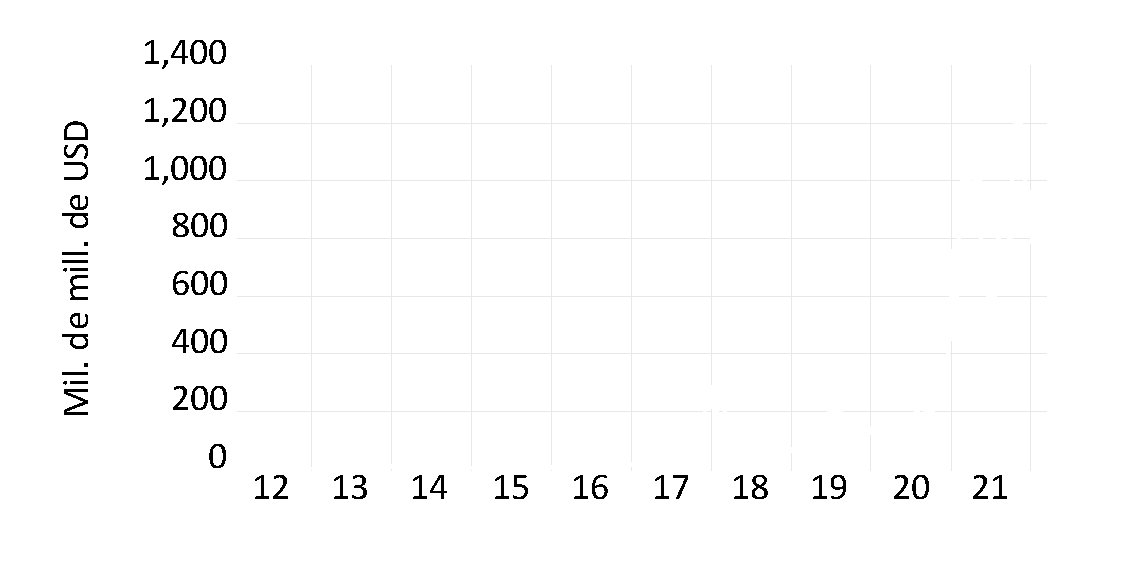
\includegraphics[width=1\textwidth]{images/C1/cap_axis.pdf}
         \end{center}
        \source{Fuente: \href{https://charts.coinmetrics.io/network-data/}{Coinmetrics}}
        \end{figure}
        \end{onlyenv}

        \begin{onlyenv}<2>
        \begin{figure}[H]
        \begin{center}
         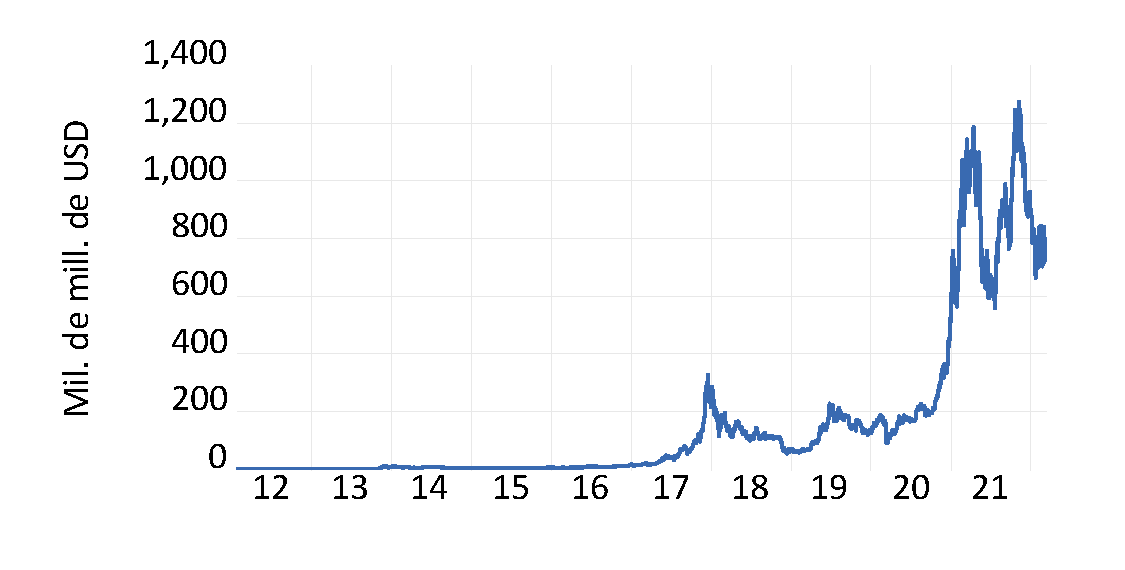
\includegraphics[width=1\textwidth]{images/C1/cap.pdf}
         \end{center}
        \source{Fuente: \href{https://charts.coinmetrics.io/network-data/}{Coinmetrics}}
        \end{figure}
        \end{onlyenv}
        
\note{
\begin{itemize}
    \item Una de las formas utilizadas habitualmente para evaluar la relevancia de bitcoin es observar la evolución en sus niveles de capitalización
    \item Valores máximos 2019: 200 mil millones de dólares aprox.
    \item Valor promedio últimos dos años: 800 mil millones de dólares aprox
    \item (900 mil millones con la suba de estos últimos días)
\end{itemize}
}
    
\end{frame}

\begin{frame}
\frametitle<1,2>{...en particular en los últimos dos años.}

        \begin{onlyenv}<1|handout:0>
        \begin{figure}[H]
        \begin{center}
         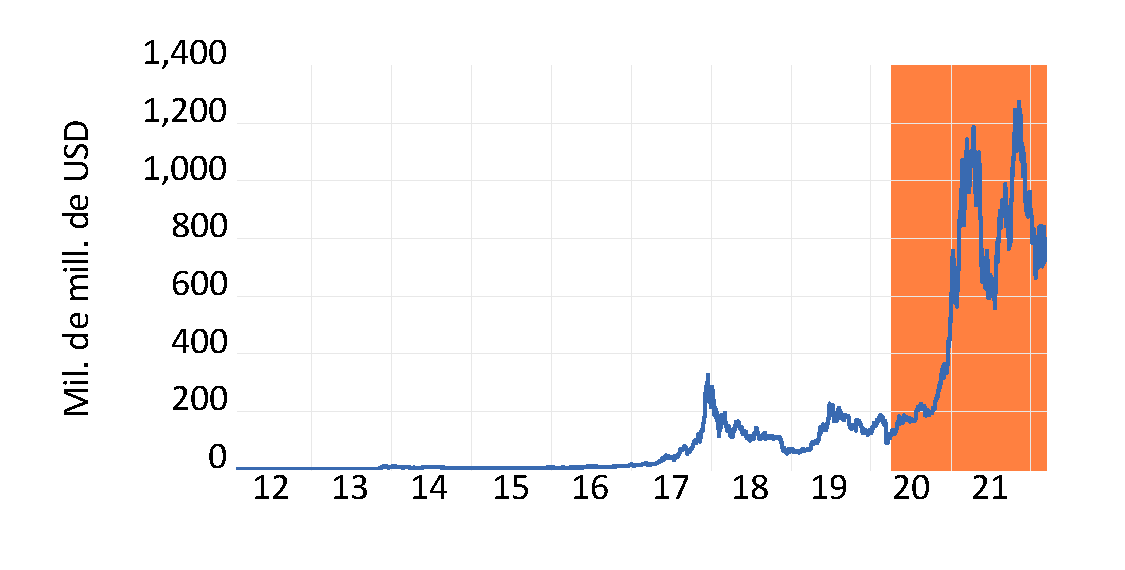
\includegraphics[width=1\textwidth]{images/C1/cap_shade.pdf}
         \end{center}
        \source{Fuente: \href{https://charts.coinmetrics.io/network-data/}{Coinmetrics}}
        \end{figure}
        \end{onlyenv}
        
        \begin{onlyenv}<2>
        \begin{figure}[H]
        \begin{center}
         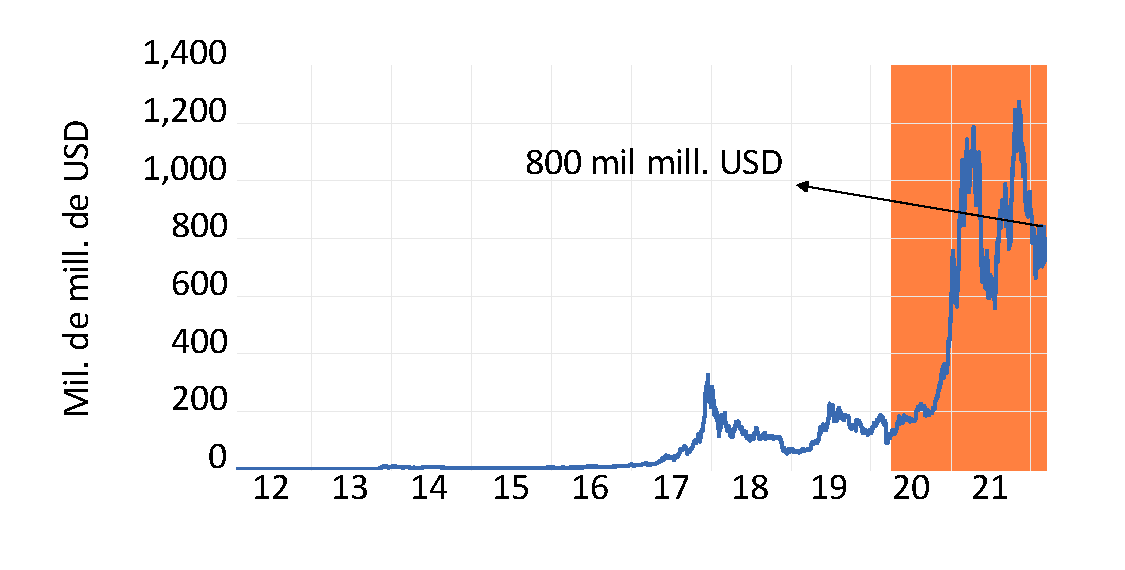
\includegraphics[width=1\textwidth]{images/C1/cap_shade_text.pdf}
         \end{center}
        \source{Fuente: \href{https://charts.coinmetrics.io/network-data/}{Coinmetrics}}
        \end{figure}
        \end{onlyenv}

\note{
\begin{itemize}
    \item 
\end{itemize}
}
    
\end{frame}

\subsubsection{Interconexiones}
%-----------------------------

\begin{frame}
\frametitle{Con relación a activos tradicionales...}

        \begin{figure}[H]
        \begin{center}
        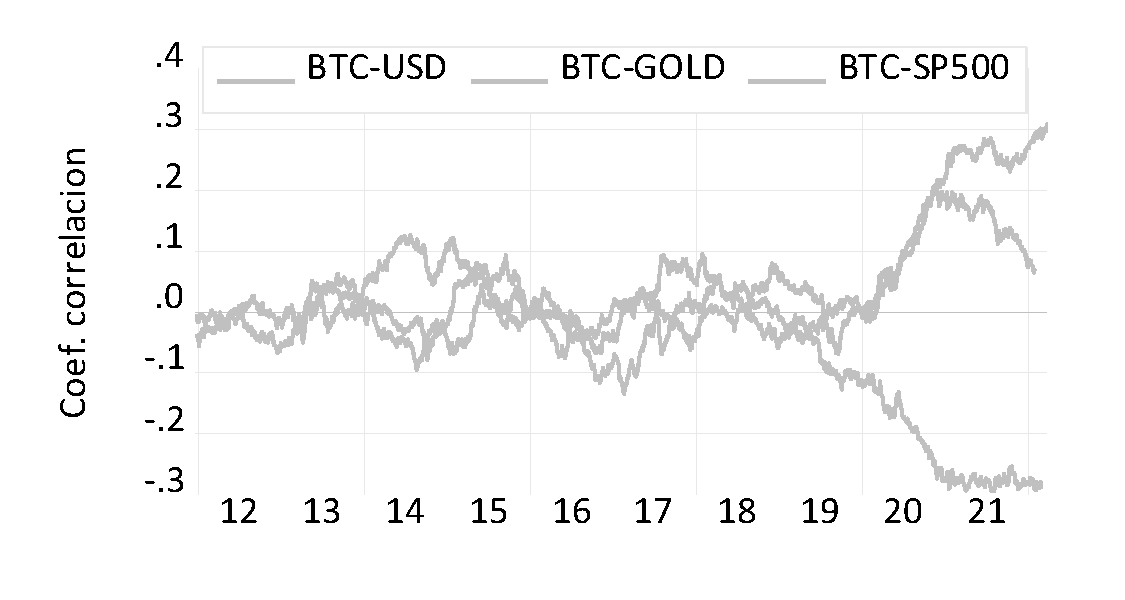
\includegraphics[width=1\textwidth]{images/C1/correlations/01.pdf}
        \end{center}
        \source{Fuente: \href{https://charts.coinmetrics.io/correlations/#435  }{Coinmetrics}}
        \end{figure}
        
\note{
\begin{itemize}
    \item Otra forma habitual de medir la relevancia de bitcoin (y ponderar sus riesgos) es buscar estimar su grado de vinculación con el sistema financiero tradicional.
    \item Por ejemplo, a través del análisis de asociación entre los rendimientos de bitcoin respecto al rendimiento de otros activos
    \item Cómo el SP500, el oro y el dólar. 
    \item \textcolor{gray}{Correlación de Spearman 360d}
    \item \textcolor{gray}{Fuente: Coinmentrics}
\end{itemize}
}
    
\end{frame}

\begin{frame}
\frametitle{... aumentó la correlación con el mercado de acciones...}

        \begin{figure}[H]
        \begin{center}
        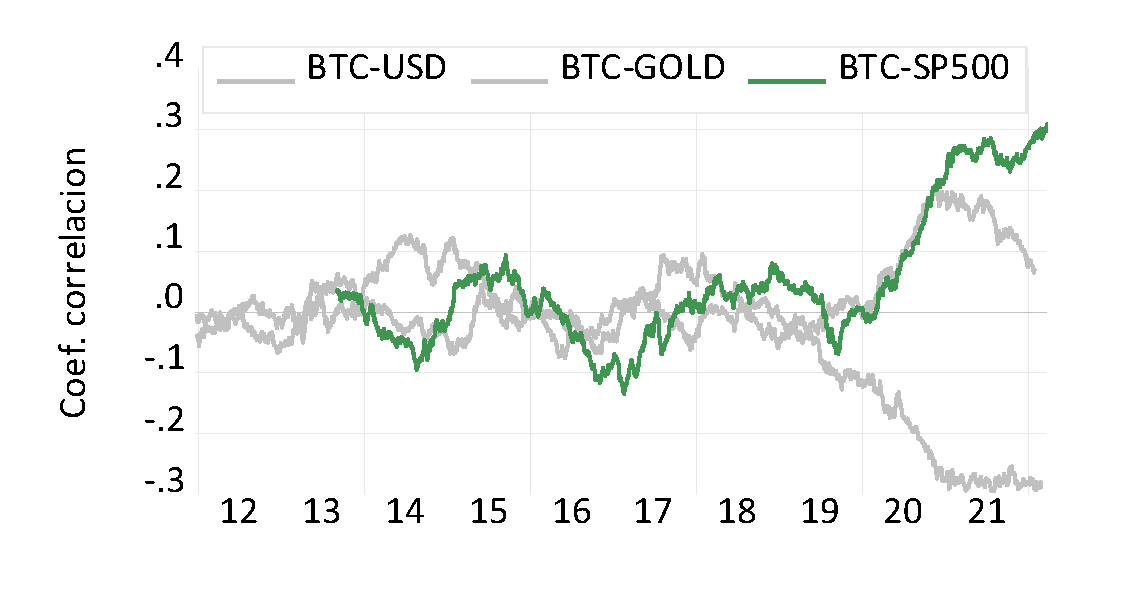
\includegraphics[width=1\textwidth]{images/C1/correlations/02.pdf}
         \end{center}
        \source{Fuente: \href{https://charts.coinmetrics.io/correlations/#3190}{Coinmetrics}} 
        \end{figure}

\note{
\begin{itemize}
    \item En los últimos dos años...
    \item ... se observa un incremento en el grado de asociación entre los rendimientos de bitcoin y el índice SP500...
    \item ... esto podría sugerir un mayor ingreso de inversores institucionales al mercado de bitcoin. 
\end{itemize}
}

\end{frame}

\begin{frame}
\frametitle{... disminuye la relación con el oro...}

        \begin{figure}[H]
        \begin{center}
        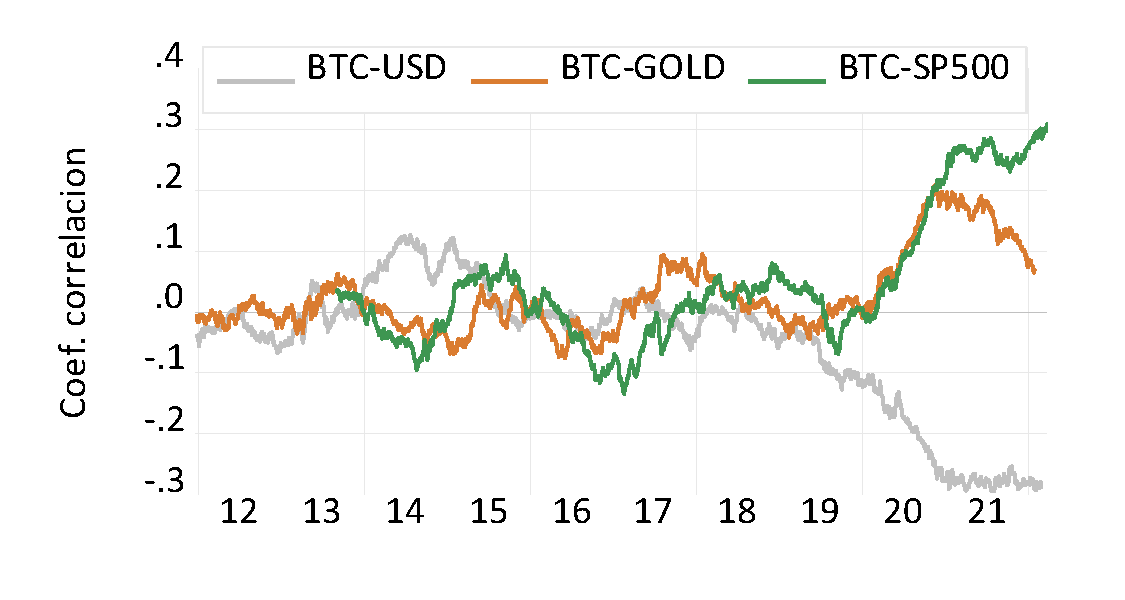
\includegraphics[width=1\textwidth]{images/C1/correlations/03.pdf}
         \end{center}
        \source{Fuente: \href{https://charts.coinmetrics.io/correlations/#3190}{Coinmetrics}} 
        \end{figure}

\note{
\begin{itemize}
    \item En el mismo período (últimos dos años)...
    \item Se observa un incremento inicial de la correlación con el oro pero luego esta correlación disminuye...
    \item ... esta situación pone en consideración las afirmaciones que sugieren que bitcoin puede situarse como un posible activo de resguardo.
\end{itemize}
}

\end{frame}

\begin{frame}
\frametitle{... y se consolida una relación negativa frente al dolar.}

        \begin{figure}[H]
        \begin{center}
        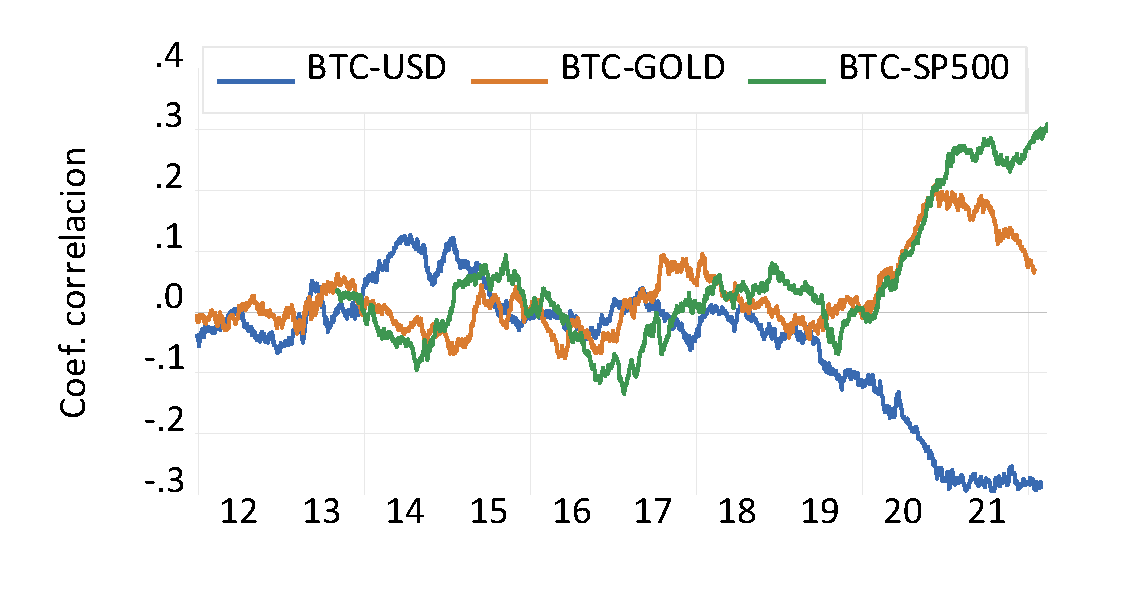
\includegraphics[width=1\textwidth]{images/C1/correlations/04.pdf}
         \end{center}
        \source{Fuente: \href{https://charts.coinmetrics.io/correlations/#3190}{Coinmetrics}} 
        \end{figure}

\note{
\begin{itemize}
    \item Finalmente, 
    \item También en el mismo período (últimos dos años)
    \item Se observa una disminución sostenida de la correlación con el índice dólar...
    \item ... esta situación podría sugerir que bitcoin puede situarse como un resguardo contra la inflación del dolar.
\end{itemize}
}

\end{frame}

\begin{frame}
\frametitle{Las entidades financieras con exposición a bitcoin se encuentra limitada}

        \begin{figure}[H]
        \begin{center}
        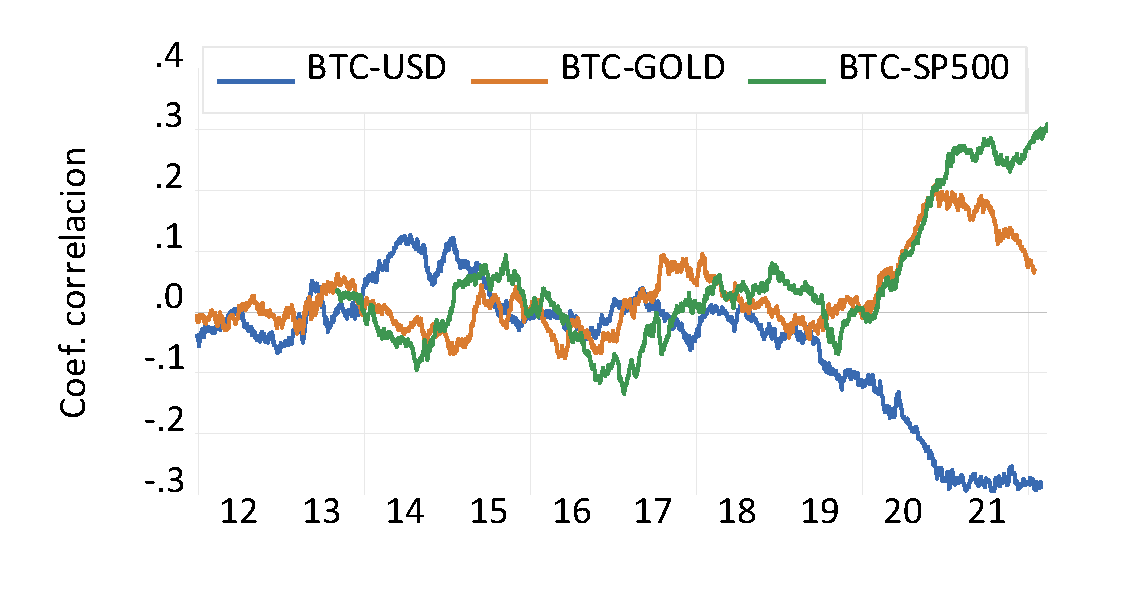
\includegraphics[width=1\textwidth]{images/C1/correlations/04.pdf}
         \end{center}
        \source{Fuente: \href{https://charts.coinmetrics.io/correlations/#3190}{Coinmetrics}} 
        \end{figure}

\note{
\begin{itemize}
    \item Finalmente, 
    \item También en el mismo período (últimos dos años)
    \item Se observa una disminución sostenida de la correlación con el índice dólar...
    \item ... esta situación podría sugerir que bitcoin puede situarse como un resguardo contra la inflación del dolar.
\end{itemize}
}

\end{frame}

\begin{frame}
\frametitle{Se incremento en la percepción de \textcolor{blue}{riesgo sistémico}..}

% slides 1/3 
\begin{columns}
    \begin{column}{0.5\textwidth}
        \begin{block}{FSB 2018}
        \begin{figure}[H]
        \begin{center}
         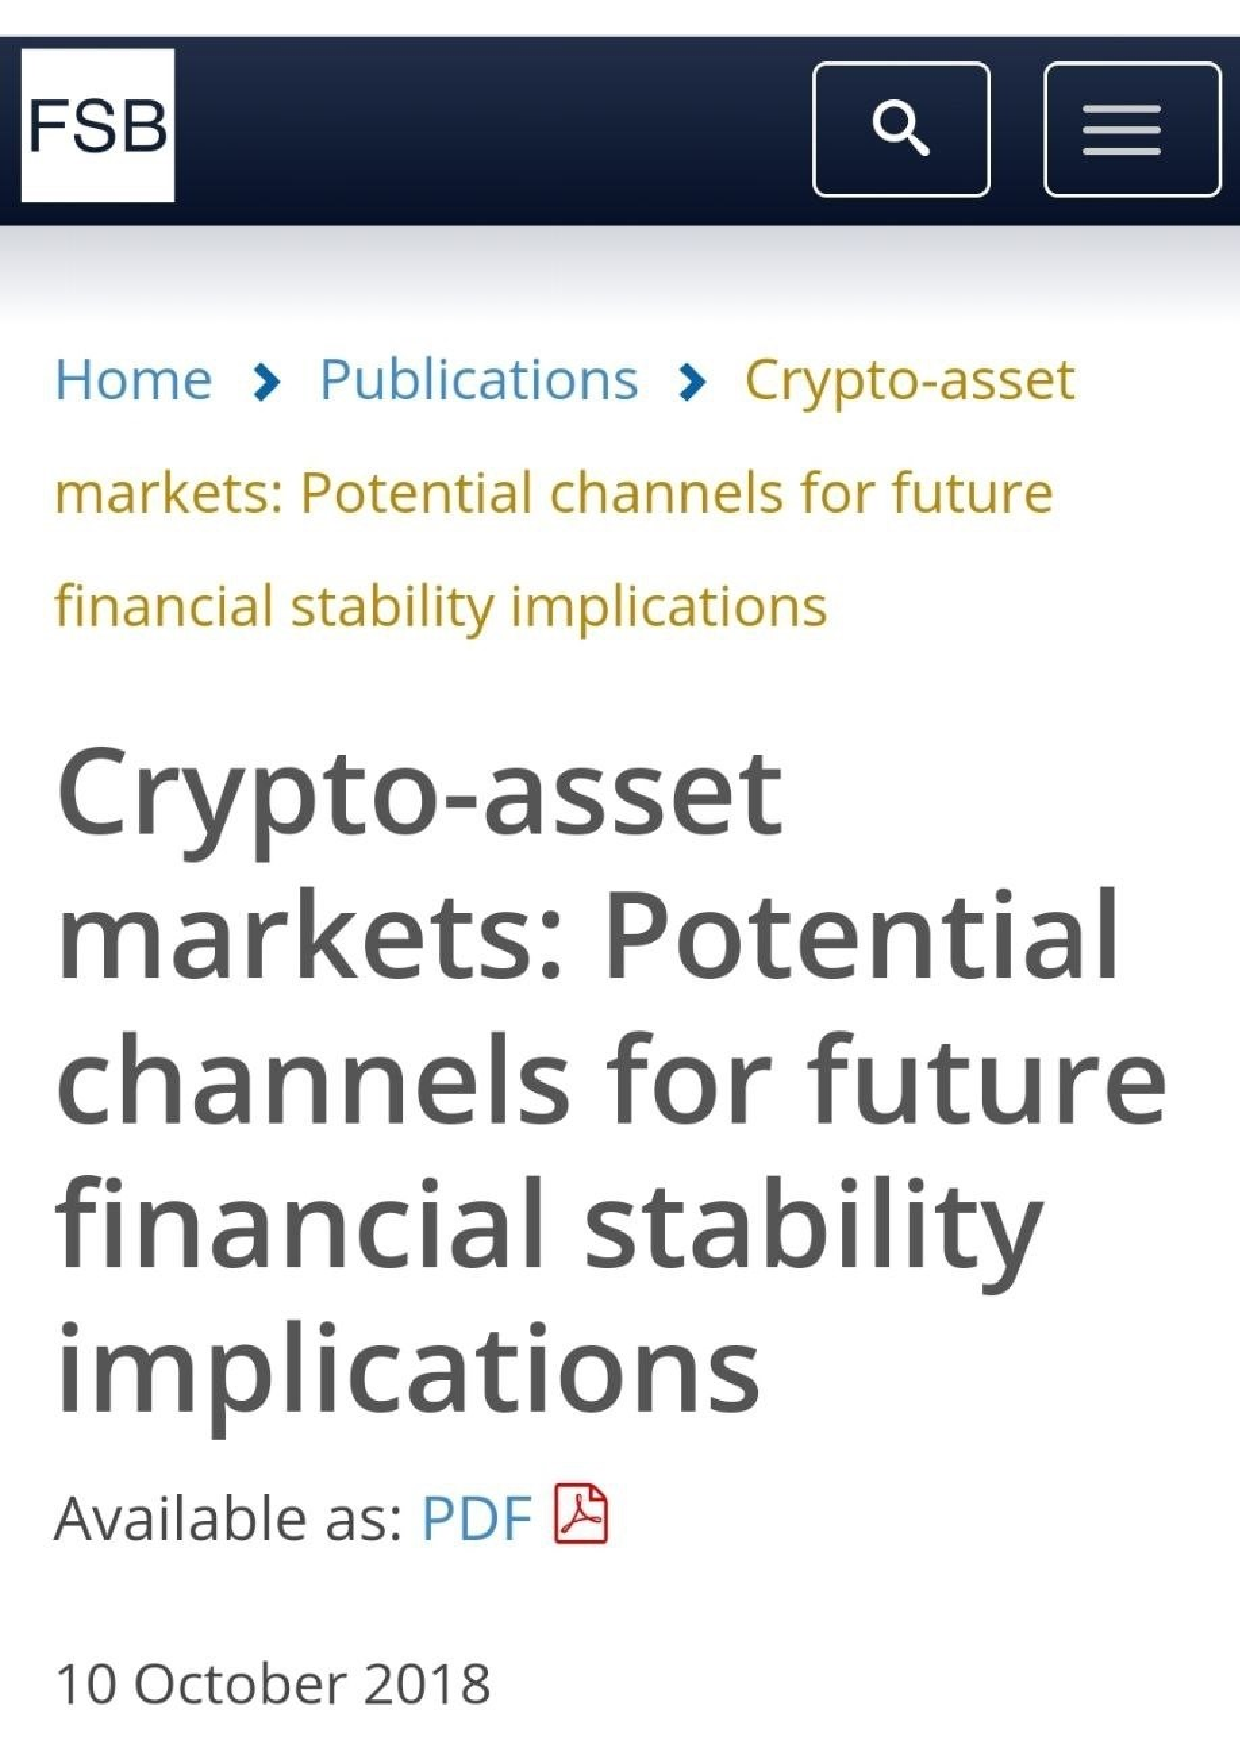
\includegraphics[width=0.6\textwidth]{images/C1/FSB 2018a.pdf}
         \end{center}
        \end{figure}
            \begin{figure}[H]
        \begin{center}
         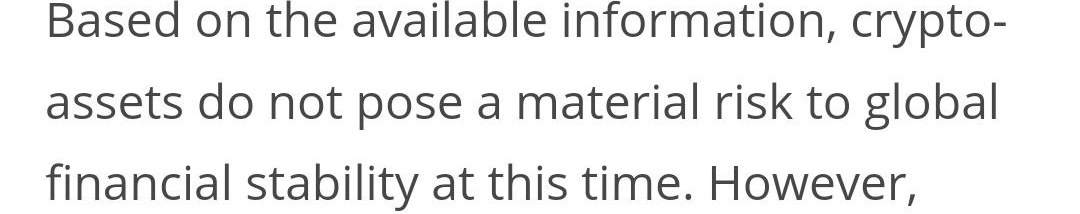
\includegraphics[width=0.8\textwidth]{images/C1/FSB 2018b}
         \end{center}
        \end{figure}
    \end{block}
    \end{column}
    \begin{column}{0.5\textwidth}  %%<--- here
        \begin{block}{FSB 2022}
        
        \begin{center}
         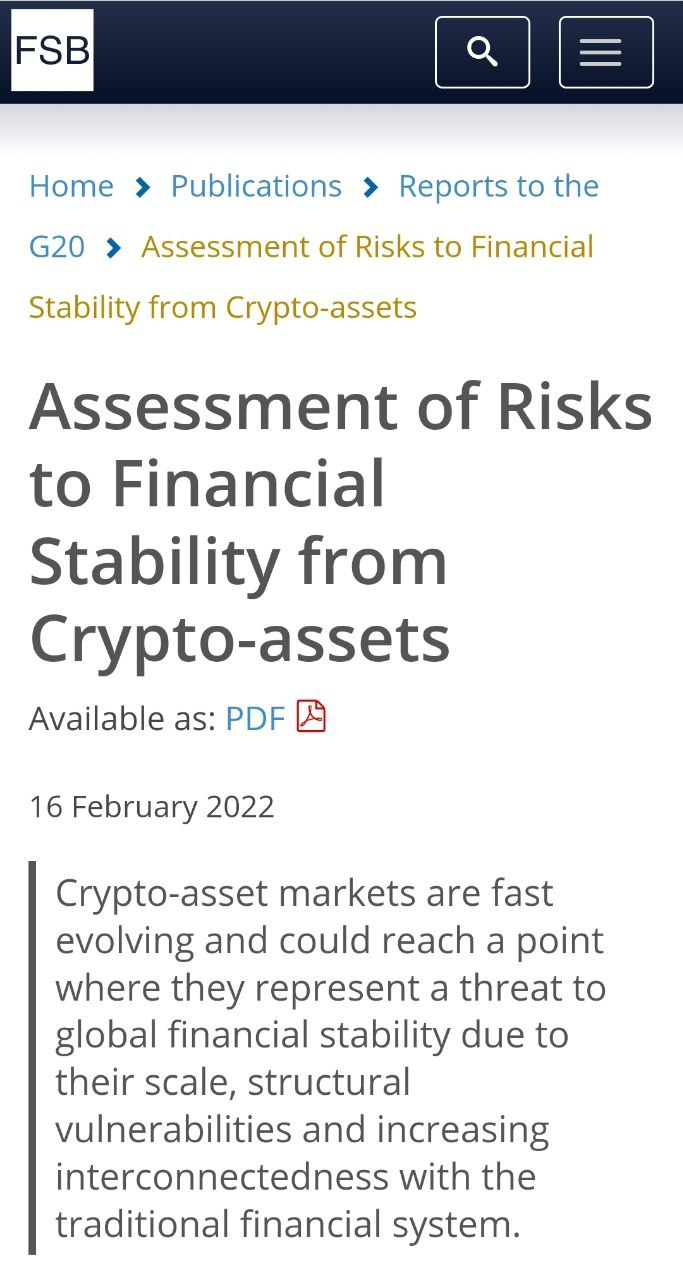
\includegraphics[width=0.6\textwidth]{images/C1/FSB 2022}
         \end{center}
             \end{block}
    \end{column}
\end{columns}

\note{
\begin{itemize}
    \item En este marco de mayor relevancia de bitcoin, se incrementa la percepción de los organismos de regulación y bancos centrales con relación a los riesgos asociados a bitcoin. 
    \item Para dar cuenta de esta posible mayor percepción del riesgo se pueden tener en cuenta, por ejemplo, las publicaciones del Consejo de Estabilidad Financiera (FSB).
\end{itemize}
}
\end{frame}
%----------

\addtocounter{framenumber}{-1}

% slides 3/3
\begin{frame}
\frametitle{...como sugieren las publicaciones del \textcolor{blue}{FSB}}

\begin{columns}
    \begin{column}{0.5\textwidth}
        \begin{block}{FSB 2018}
        
        \pgfsetfillopacity{0.4}% transparencia
    
         \begin{figure}[H]
        \begin{center}
         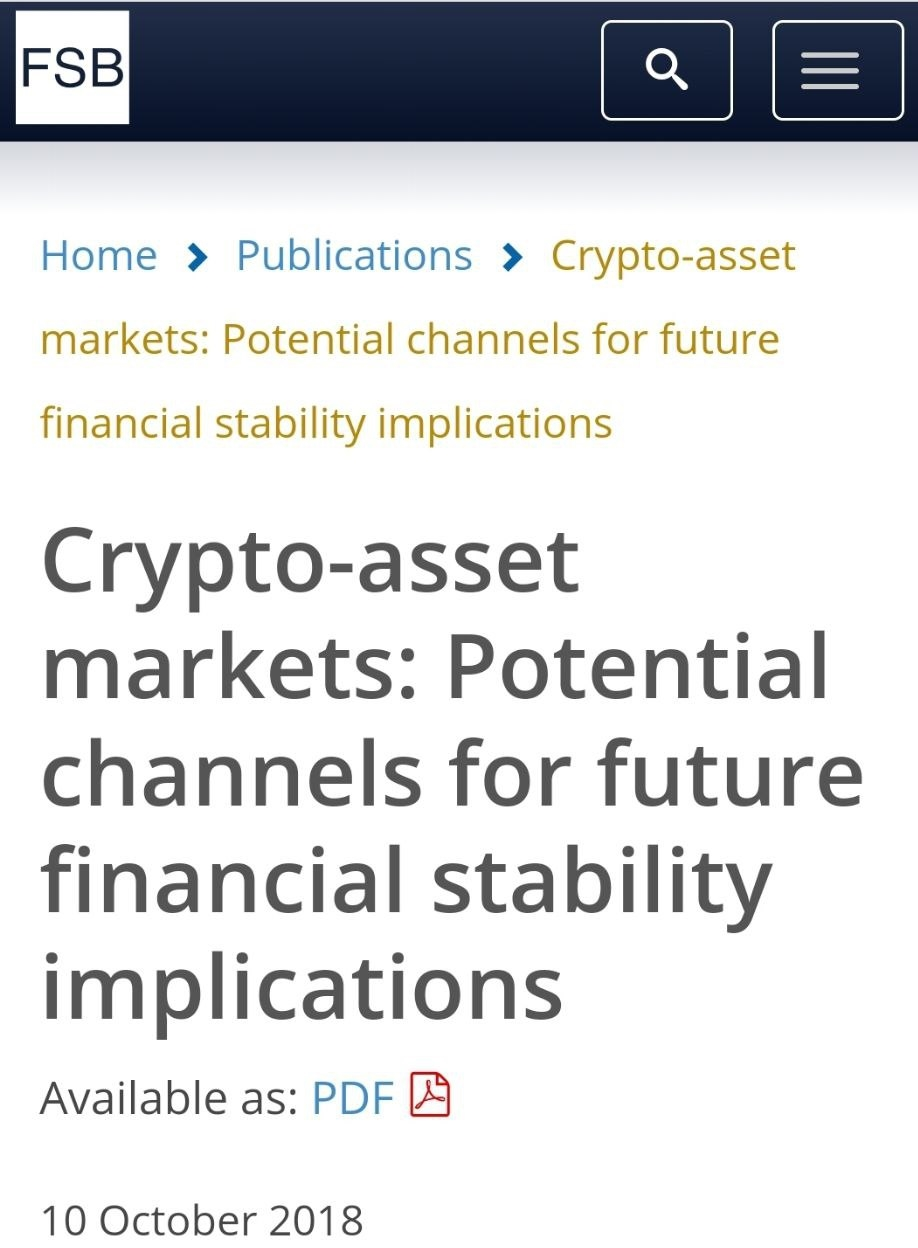
\includegraphics[width=0.6\textwidth]{images/C1/FSB 2018a}
         \end{center}
        \end{figure}
            \begin{figure}[H]
        \begin{center}
         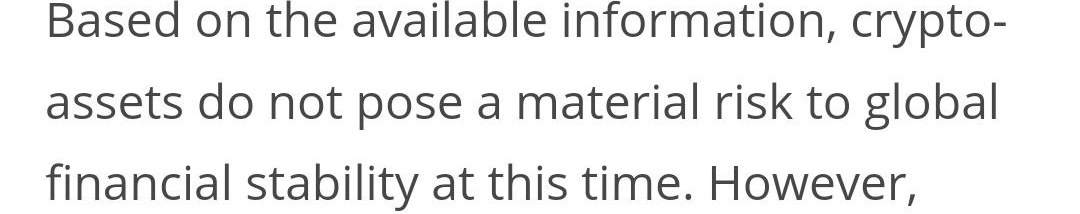
\includegraphics[width=0.8\textwidth]{images/C1/FSB 2018b}
         \end{center}
        \end{figure}
    \end{block}
    
    \pgfsetfillopacity{1}% transparencia
    
    % overlay 2018
        \begin{tikzpicture}[overlay][t] 
         \node[anchor=north east,xshift=5.5cm,yshift=2
         cm]{ 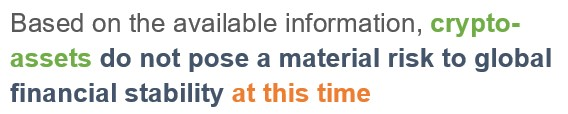
\includegraphics[width=1\textwidth]{images/C1/FSB 2018b overlay.jpg}};
        \end{tikzpicture}
    
    \end{column}
    \begin{column}{0.5\textwidth}  %%<--- here
        \begin{block}{FSB 2022}
        
        \pgfsetfillopacity{0.4}% transparencia
        
        \begin{center}
         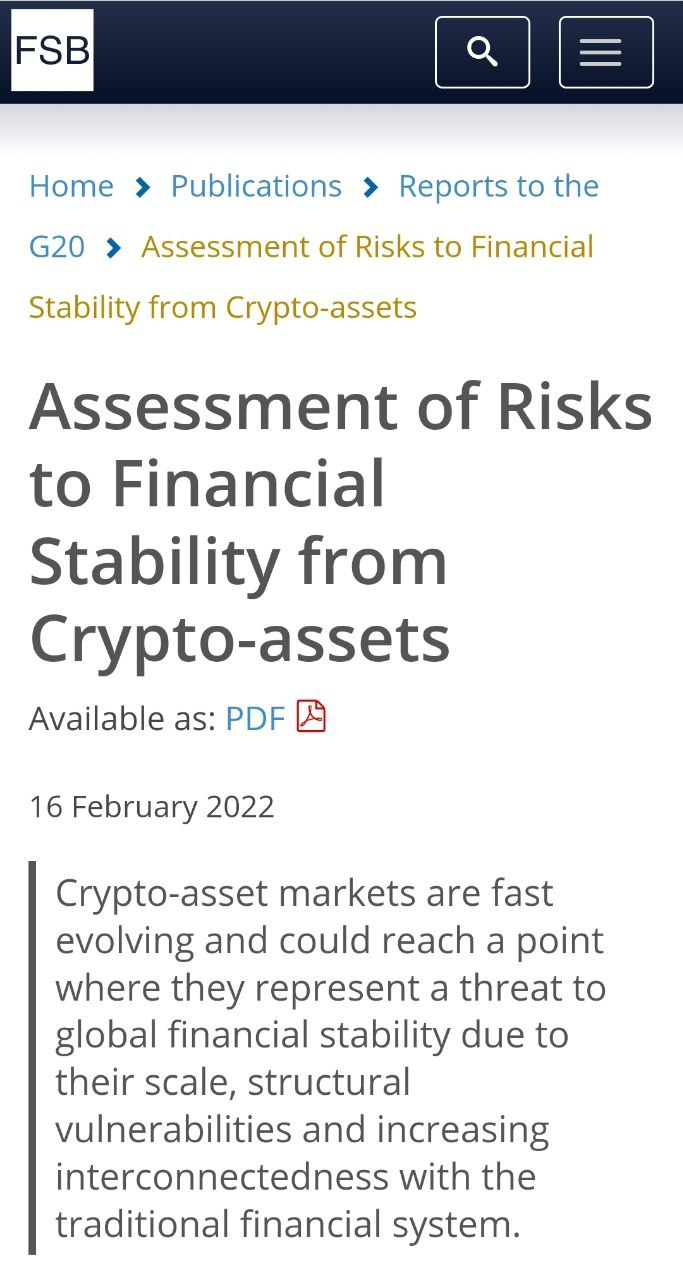
\includegraphics[width=0.6\textwidth]{images/C1/FSB 2022}
         \end{center}
             \end{block}
             
        \pgfsetfillopacity{1}% transparencia
             
        % overlay 2022
        \begin{tikzpicture}[overlay][t] 
         \node[anchor=north east,xshift=5.5cm,yshift=2.5
         cm]{ 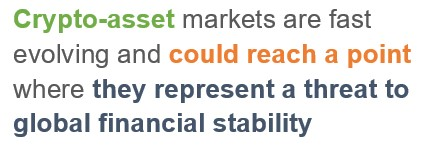
\includegraphics[width=0.9\textwidth]{images/C1/FSB 2022 overlay.jpg}};
        \end{tikzpicture}
             
    \end{column}
    
\end{columns}

\note{
\begin{itemize}
    \item Si se comprara, por ejemplo, la primera publicación del FSB respecto a la última (de febrero de este año), se encuentran conclusiones diferentes:
    \item 2018: "Basado en la información disponible, \textbf{los criptoactivos no suponen en ese momento un riesgo para la estabilidad financiera global}"
    \item 2022: "Los mercados de criptoactivos están evolucionando rápidamente y \textbf{podrían llegar a representar una amenaza para la estabilidad financiera mundial"}
\end{itemize}
}
\end{frame}
%----------

% IMF y BOE

\begin{frame}
\frametitle{... y las publicaciones del \textcolor{blue}{IMF} y el \textcolor{blue}{BoE} ...}

% slides 1/3 
\begin{columns}
    \begin{column}{0.5\textwidth}
        \begin{block}{BoE 2021}
        \begin{figure}[H]
        \begin{center}
         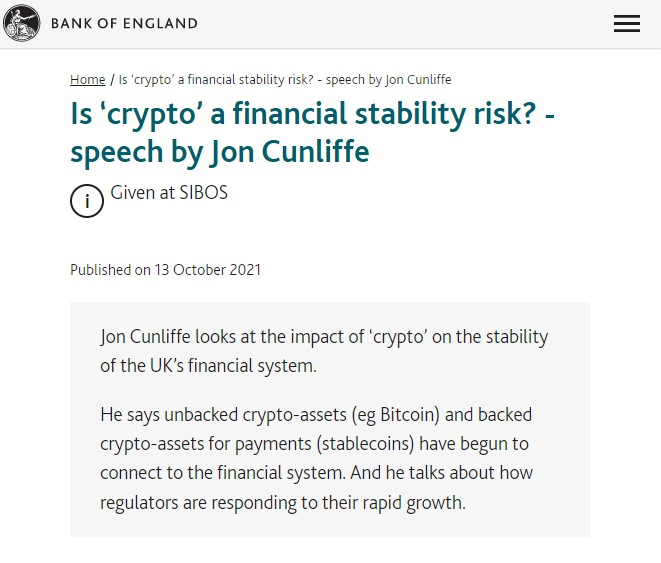
\includegraphics[width=1\textwidth]{images/C1/global/BoE 2021.jpg}
         \end{center}
        \end{figure}
              \end{block}
    \end{column}
    \begin{column}{0.5\textwidth}  %%<--- here
        \begin{block}{IMF 2021}
        \begin{center}
         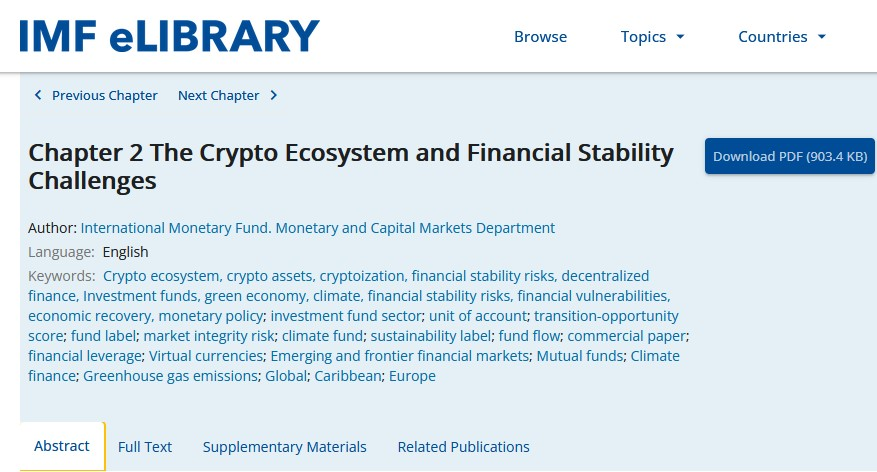
\includegraphics[width=1\textwidth]{images/C1/global/IMF 2021d.jpg}
         \end{center}
             \end{block}
    \end{column}
\end{columns}

\note{
\begin{itemize}
\item En el mismo sentido se encuentran las últimas publicaciones del BoE y del IMF (a través de su GFSR)
\end{itemize}
}
\end{frame}
%----------

%-------------------------------
\subsection{Relevancia local}
%-------------------------------

\subsubsection{Oferta}
%------------------

\begin{frame}
\frametitle<1,2>{A nivel \textcolor{blue}{local} se expande la \textcolor{dgreen}{oferta}...}

    \begin{figure}
    \centering
        \includegraphics<1>[width=1\textwidth]{images/C1/arg/bloomberg (1).jpg}
        \includegraphics<2|handout:0>[width=1\textwidth]{images/C1/arg/afa.jpg}
        \vspace{-5mm}
        \caption*{Fuente: \href{https://www.bloomberg.com/news/articles/2022-03-09/cryptocurrencies-prove-a-lifeline-in-argentina-s-chaotic-economy}{Bloomberg}}
    \end{figure}
    
    \note{
    \begin{itemize}
        \item A nivel local, 
        \item Se observa una creciente oferta de proveedores de bitcoin
        \item Como reflejan estas publicidades de operadores locales en la vía pública
        \item Fuente: Bloomberg
        \item nota vinculada a la reciente regulación del BCRA https://www.ft.com/content/4dae4742-c339-4414-9bfa-4739df6e5248
    \end{itemize}
    }
    
\end{frame}
%----------

\subsubsection{Demanda}
%------------------

\begin{frame}
\frametitle{A la vez que se incrementa la \textcolor{dgreen}{demanda}...}
    \begin{figure}
    \centering
        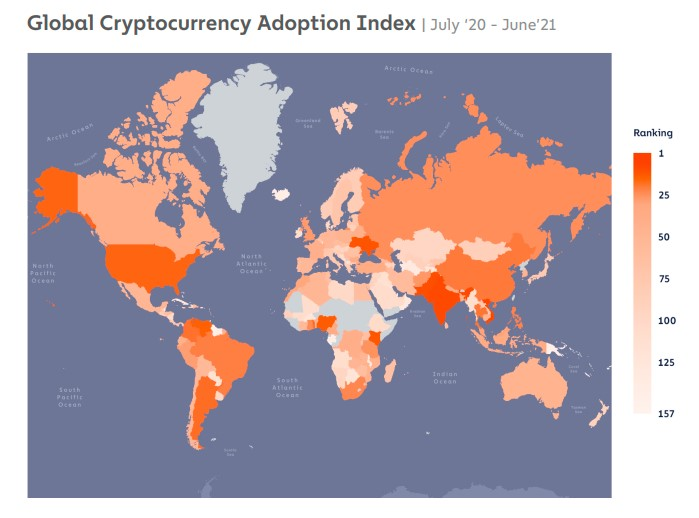
\includegraphics[width=0.8\textwidth]{images/C1/arg/arg_demanda (1).jpg}
        \caption*{Fuente: \href{https://blog.chainalysis.com/reports/2021-global-crypto-adoption-index/}{Chainalysis}}
        \end{figure}
        
    \note{
    \begin{itemize}
        \item Al mismo tiempo que se incrementa la oferta se puede identificar un incremento en la demanda.
        \item Se puede dar cuenta de este incremento en la demanda por, por ejemplo, a través del índice de adopción global de la empresa Chainalysis ...
        \item ... de octubre 2021 ...
        \item ... donde Argentina figura en el número 10° (primer país en AL, Brasil 14°).
    \end{itemize}
    }

\end{frame}

\begin{frame}
\frametitle{... en particular \textcolor{blue}{p2p}}.

    \begin{figure}
    \centering
        \includegraphics<1>[width=0.8\textwidth]{images/C1/global/IMF 2021b.jpg}
        \includegraphics<2>[width=0.8\textwidth]{images/C1/global/IMF 2021b - copia.jpg}
        \vspace{-5mm}
        \caption*{Fuente: \href{https://www.imf.org/-/media/Files/Publications/GFSR/2021/October/English/ch2.ashx}{IMF (2021) GFSR}}
        \end{figure}
        
    \note{
    \begin{itemize}
        \item Este incremento en la demanda se observa con particular énfasis en las operaciones directas entre personas (p2p)
        \item Estos datos son tomados del GFSR del IMF de octubre de 2021. 
        \item ... donde Argentina 5° Binance. 
    \end{itemize}
    }

\end{frame}

\begin{frame}
\frametitle{... en particular \textcolor{blue}{p2p}}.

    \begin{figure}
    \centering
        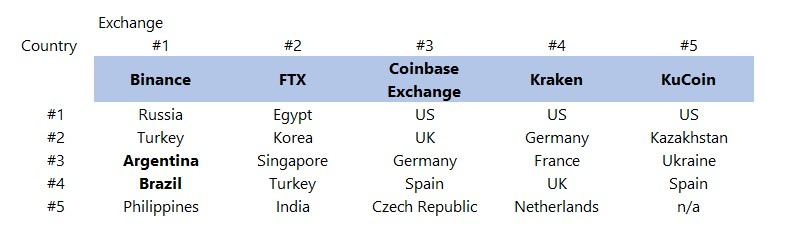
\includegraphics[
        [width=0,scale=0.55]{images/C1/global/p2p.jpg}
        \vspace{5mm}
        \caption*{Fuente: \href{https://www.similarweb.com/es/}{Similarweb}}
        \end{figure}
        
    \note{
    \begin{itemize}
        \item 
    \end{itemize}
    }

\end{frame}

\begin{frame}
\frametitle{Ranking de precios de compra y venta local}.

    \begin{figure}
    \centering
        \includegraphics<1>[width=1\textwidth]{images/C1/arg/coinmonitor.jpg}
        \caption*{Fuente: \href{https://www.coinmonitor.info/}{CoinMonitor Argentina}}
        \end{figure}
        
    \note{
    \begin{itemize}
        \item La oferta y demanda de bitcon local se puede sintetizar en el cuadro con el RANKING DE LOS MEJORES PRECIOS FINALES -comisiones incluídas- DE LOS PRINCIPALES BROKERS O EXCHANGES DE INTERES EN ARGENTINA 
        \item de la página local "CoinMonitor"
        \item aproximadamente 15 operadores
    \end{itemize}
    }

\end{frame}

%----------------------------------
\subsection{Taxonomía/clasificación}
%-----------------------------------

\begin{frame}
\frametitle{De manera preliminar, la taxonomía de criptoactivos es la siguiente}.

    \begin{figure}
    \centering
        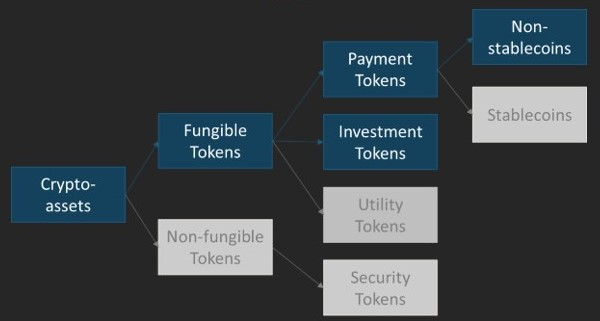
\includegraphics[width=1\textwidth]{images/C1/classification/classification.jpg}
        \caption*{Fuente: elaboración propia en base a IMF}
        \end{figure}
        
    \note{
    \begin{itemize}
        \item 
    \end{itemize}
    }

\end{frame}

%---------------------
\subsection{Preguntas}
%---------------------

\begin{frame}

\Large
\centering
¿Un incremento en la demanda de bitcoin en Argentina puede afectar la estabilidad financiera?

    \note{
    \begin{itemize}
        \item En ese marco de aumento de la relevancia de bitcoin en particular en los últimos dos años...
        \item ... se plantea la pregunta general de la investigación:
        \item ¿Un incremento en la demanda de bitcoin ...?
    \end{itemize}
    }
    
\end{frame}
%----------

\begin{frame}

\begin{itemize}
    \item[] \onslide<1>{\textcolor{blue}{\textbf{Oferta}}}
    \item[] \onslide<2>{¿Es posible que \textcolor{blue}{bitcoin} puede funcionar como una \textcolor{blue}{tecnología equivalente al dinero}?}
    
    \vspace{5mm}
    \item[] \onslide<1>{\textcolor{dgreen}{\textbf{Demanda}}}
    \item[] \onslide<3>{¿Es posible que la \textcolor{dgreen}{demanda de bitcoin} se encuentre asociada a las opiniones de un grupo de \textcolor{dgreen}{actores influyentes}?}
    
    \vspace{5mm}
    \item[] \onslide<1>{\textcolor{orange}{\textbf{Implicancias}}}
    \item[] \onslide<4>{¿Un \textcolor{orange}{mayor} nivel de \textcolor{orange}{adopción} de bitcoin puede generar incrementos en la \textcolor{orange}{volatilidad del tipo de cambio} entre pesos y dólares en Argentina?}
\end{itemize}

    \note{
    \begin{itemize}
        \item Para responder a esa pregunta general, se proponen \textbf{tres preguntas específicas}. 
        \item Las dos primeras se vinculan al análisis del mercado de oferta y demanda de bitcoin.
        \item La última se asocia a las implicancias de un mayor grado de adopción de bitcoin en Argentina. 
        \item Las preguntas específicas son: ..., ..., ...
    \end{itemize}
    }
    
\end{frame}

%---------------------
\subsection{Overviews}
%---------------------

%-----------------------------------------------------
\subsubsection{Perspectiva general de la investigación}
%-----------------------------------------------------

\begin{frame}
\frametitle{Perspectiva general}
%------------------------------
\begin{columns}

    \begin{column}{0.50\textwidth}
    \vspace{-5pt}
    \begin{block}{\textcolor{blue}{Oferta}}
        \begin{column}{0.1\textwidth}
        \vspace{-10pt} % estos espacios negativos son claves para alinear
            \tiny
            \begin{align*}
            c_{1,t}+\Phi_t \le y\\
            c_{2,t+1}\le\Phi_{t+1}^R\\
            N_{t-1}\textcolor{red}{x_t} \cdot \Phi_{t-1}^{\textbf{DLT}}=N_t(*)
            \end{align*}
        \end{column}
        \begin{column}{0.35\textwidth}  
            \begin{figure}[H]
            \begin{center}
             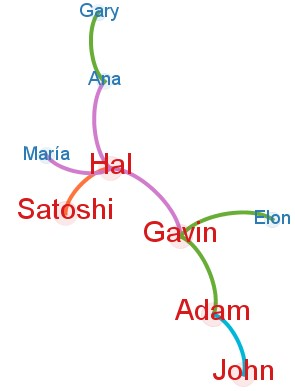
\includegraphics[width=1\textwidth]{images/C2/c2_simul_red5.jpg}
             \end{center}
            \end{figure}
            \end{column}
    \end{block}
    \begin{block}{\textcolor{dgreen}{Demanda}}
        \vspace{-10pt}
            \tiny
              \begin{align*}
              v_{t}^{\$}{M_{t}^{\$}}&={N_{t}^{\$}\left(*\right)}+(1-\lambda_t){N_{t}^{\$}\left(*\right)}\\
              v_{t}^{\bitcoinA}{M_{t}^{\bitcoinA}}&={N_{t}^{\bitcoinA}\left(*\right)+\lambda_tN_{t}^{\$}\left(*\right)}\\
              \lambda_t&=\textcolor{blue!70}{S}(\textcolor{red}{\mu_t})
            \end{align*}
    \vspace{-20pt}
            \begin{figure}[t!]
            \begin{center}
            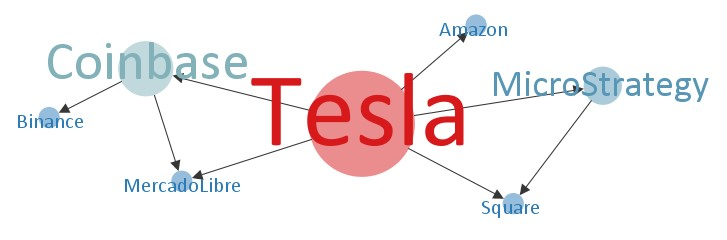
\includegraphics[width=0.6\textwidth]{images/C3/c3_simul_influ3.jpg}
             \end{center}
            \end{figure}
            
    \end{block}
    \end{column}
    
    \begin{column}{0.55\textwidth}
    
    \begin{block}{\textcolor{orange}{Implicancias}}
    \tiny

    \begin{align*}
    v^{\$a}_1 M^{\$a}_1&=P_1^{{\$a}} + \lambda_1 (1-\alpha_1) R_1^{{\$a}} + (1-\lambda_1) \textcolor{blue!60}{\rho_1}  R_1^{{\$a}}\\
    v_1^{\$} M_1^{\$}&=(1-\lambda_1) \textcolor{green!70}{\delta_1} R_1^{\$a}\\
    v_1^{\bitcoinA} M_1^{\bitcoinA}&=\textcolor{orange}{\lambda_1}  \alpha_1 R_1^{\$a} + (1-\lambda_1) \textcolor{red}{\beta_1} R_1^{\$a}\\
    e_t^{{\$a};{\$}}&=\frac{v_1^{\$a}}{v_1^{\$}}
    \end{align*}
    
    \vspace{-5pt}
    
    \begin{figure}[H]
    \begin{center}
     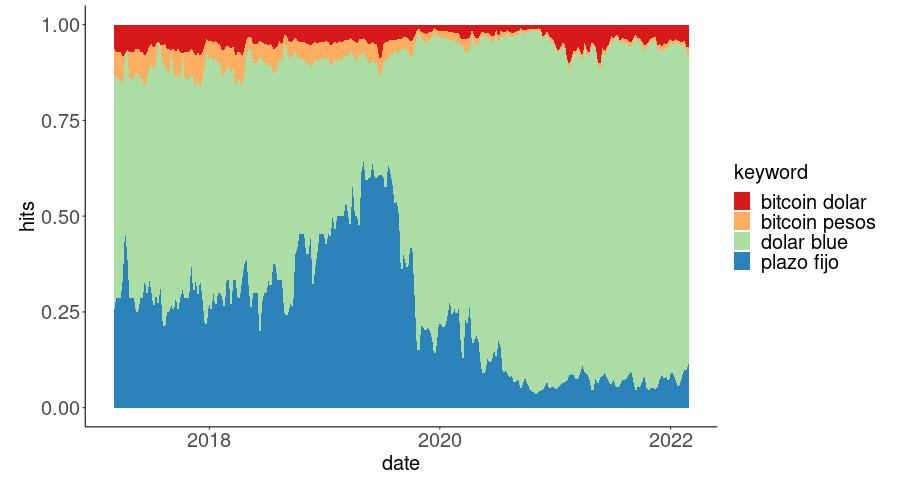
\includegraphics[width=1\textwidth]{images/C4/Rplot001.png}
     \end{center}
    \end{figure}
    
    \end{block}

    \end{column}
\end{columns}

\note{
\begin{itemize}
    \item Para poder dar respuestas a cada una de dichas preguntas se propone una evaluación conceptual y una evaluación empírica. 
    \item Evaluación conceptual
        \begin{itemize}
        \item Modelos OLG para los tres objetivos, con el mismo entorno (previsión perfecta, estacionariedad, un solo bien, dos generaciones que viven dos períodos, tiempo infinito).
        \end{itemize}
    \item Evaluación empírica
        \begin{itemize}
        \item Objetivo 1 y 2: técnicas de análisis de red
        \item Objetivo 3: datos de Google Trend (no hay posibilidad de georeferenciar datos de la blockchain o Twitter).
        \end{itemize}
\end{itemize}
}

\end{frame}
%----------


